%As part of evaluation, we used rcu torture test. It provides support for testing all rcu implementations and gets enabled by config option CONFIG\_RCU\_TORTURE\_TEST. It creates an rcutorture kernel module that can be loaded to run torture test.  The test periodically outputs status messages via printk(), which can be examined via dmesg. The test gets started when the module is loaded, and stops when the module is unloaded. We verified our system by running it in a Guest virtual machine hosted by system equipped with an Intel(R) Core(TM) i7-860X 2.80 GHz CPUprocessor. In the course of evaluation all system was running Linux 2.6.32 kernel.
%As part of evaluation, we used microbenchmark and RCU torture test to determine the overhead posed by 
%\subsection{Hypothesis}
%Our evaluation strategy aims to test the following hypotheses:
Our evaluation strategy tests the following:
\begin{enumerate}
	\item[i)] The performance overhead of Granary and Watchpoint used for debugging incorrect usage of RCU primitives.
	\item[ii)] Dynamic Binary Instrumentation (DBI) can be used to debug the incorrect usage of RCU primitives.
	\item[iii)] The space overhead of shadow memory used for storing contextual information.
\end{enumerate}

\subsection{Performance Overhead}
\begin{figure}
\centering
 	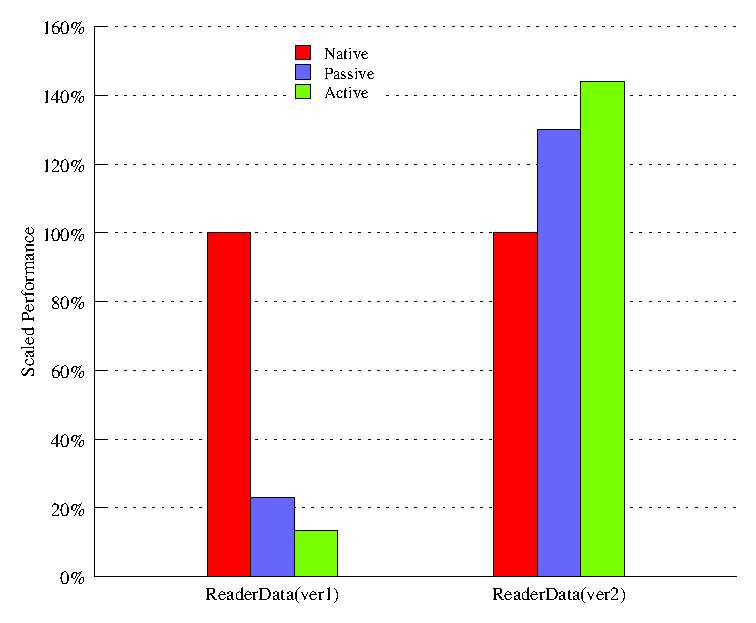
\includegraphics[width=0.45\textwidth]{rcu_rw}
\caption{Scaled performance of Reader thread in terms of ages of structures it sees. With instrumented code there is a decrease in flip counts for which reader sees the current data and increase in the flip counts for which it sees the old version}\label{fig:perf}
\end{figure}
We evaluated the performance of behavioural watchpoints using a microbenchmark and RCU tortute test (with 10 readers and 5 writers) by running them in three different execution modes: Native, Passive and Active mode. Passive and Active execution both run the Granary DBI framework; however, passive execution only performs basic translation of module code, while active execution translates and adds watchpoint-specific instrumentation to module code, actively looking for watchpoints.%The Passive mode implies the system running with null instrumentation and Active mode implies the system running with watchpoint instru  
Our tests ran on a desktop equipped with an Intel\textregistered\ Core\texttrademark\ E7500 2.93 GHz CPU, 4GB memory, and an Intel 82598EB  10-Gigabit Ethernet card. %Watchpoint instrumentation was enabled for every memory load and store, and 
For testing with \texttt{rcutorture} module, Watchpoints were active for all RCU protected memory allocated from the memory pool.

\paragraph{Microbenchmark} The microbenchmark performed a tight-loop of memory operations on watched addresses and exhibits the worst-case performance overhead of watchpoints (about 20{\footnotesize$\times$}). This is expected because our instrumentation adds instructions to each memory load and store.
 %added to all memory returned from kernel heap allocators. 
%To evaluate the performance overhead incurred by the Granary and watchpoint we used rcutorture module running with 100 reader and 5 writer threads. As experimental setup, we run our system in Guest Virtual machine (QEMU) running with four core and powered with Linux 2.6.32 kernel on a Host system equipped with an Intel(R) Core(TM) i7-860, 2.80 GHz CPU. Our evaluation strategy involves running rcutorture module natively, under the control of Granary \& Granary with watchpoint active and studying the following parameters :
%\paragraph{\texttt{rcutorture}} We tested the \texttt{rcutorture} kernel module. It exhibited interesting behaviour: all threads experienced a minimum of 6{\footnotesize$\times$} overhead; however, readers were abnormally penalized and tended to see more stale data. We think this is because each writer synchronized with fewer readers.
\paragraph{RCU tortute test} we evaluated our system using \texttt{rcutorture} module running with 10 readers and 5 writers. We run the test in all the three execution mode to study the following parameters: %To run the RCU torture test, we enabled the \texttt{CONFIG\_RCU\_TORTURE\_TEST} config and build the \texttt{rcutorture} module. %We testedWe tested the performance overhead incurred by Granary and watchpoints using \texttt{rcutorture} kernel module. Our evaluation strategy involves running rcutorture module natively, under the control of Granary \& Granary with active watchpoints and studying the following parameters :
\begin{enumerate}
	\item[i)] \emph{Ver:} The number of times RCU writer task has changed the structure visible to readers.
	\item[ii)] \emph{Readers Batch:} Histogram of ages of structure seen by the readers in terms of \emph{counter flips}.
\end{enumerate}
We recorded these parameters by running the module for 60 sec and averaged it over five different runs. 
%The Reader Batch histogram of the \texttt{rcutorture} module shows the performance of readers thread. 
In our observation to Reader Batch histogram, we found an interesting behaviour: all threads experienced a minimum of 7{\footnotesize$\times$} overhead, which is evident from the fact that the age of current structure seen by reader decreases. We also found that the readers were abnormally penalized and tended to see more stale data. \Figref{perf} shows the behaviour of reader thread when tested in three different execution modes. 

The interesting observation we made while testing the system in all three execution mode is that the performance overhead is not much because of watchpoints. There is a significant drop in the performance of readers when rcutorture is run in Passive execution mode. One reason for this could be the annotations we used for all read side primitive to make a callback to kernel wrapper. These kernel wrapper runs natively and are not in code-cache. There is a cost involved when Granary switches execution from the code-cache to native since it has to switch the stack and save and restore the machine context. We have seen similar behaviour earlier with other file-system modules while running benchmarks like postmark~\cite{katcher97postmark} which involves many context switches. To verify this we removed the annotation and tested the \texttt{rcutorture} module in Passive execution mode but we didn't get any improvement. We also found similar behaviour when tested with DynamoRIO kernel(DRK) instrumenting entire kernel code. One reason for this could be the design of DBI framework, which mainatains per-cpu codecache and not very friendly for analysing parallel programs.    %We have not yet verified this with rcutorture module.  

\begin{figure}
\centering
 	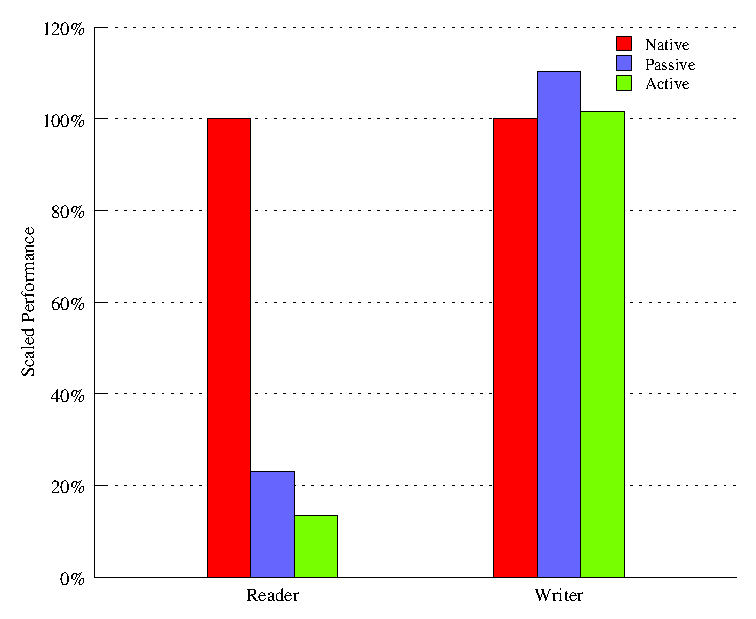
\includegraphics[width=0.45\textwidth]{rcu}
\caption{Scaled performance of reader and writer thread. The performance of readers decreases but there is an increase in the number of times writer thread getting scheduled.}\label{fig:reader-writer}
\end{figure}
We made another interesting observation while comparing the performance of writer thread and found its unusual behaviour when run under Passive and Active execution mode. \Figref{reader-writer} shows the increase in the performance of writer thread when run in Passive mode. In this case also the behaviour was same when tested with DynamoRIO kernel(DRK). We used \emph{Ver} parameter to get the writer performance which counts the number of times write thread getting scheduled. We are investigating the reason for such behaviour. 
%We also studied the performance of writer thread by using the \emph{Ver} parameter as referred in \Figref{reader-writer}.  

%We think this is because each writer synchronized with fewer readers.
  %Table~\ref{table:nonlin} below shows these parameters for three different cases. Our experimental result shows moderate decrease in ver number which shows the number of times writer task has changed the structure visible to readers but there is a drastic decrease in the readers \emph{Readers Pipe} and \emph{Readers batch} showing the increase in the readers seeing stale data. We think this is because each writer synchronized with fewer readers. The performance of readers and writers based on these parameters is shown in figure~\ref{fig:perf}.
% The result shows a moderate decrease in the performance of writer but the performance of readers decreases by approximately 10 times. One of the reason for this is we are testing the system with 100 readers but only 5 writers thread and read is the most frequent operation in the rcu torture test. Our system also instrument both memory read and write which is going to be costly but it gets amortized over the large number of instructions.

%\begin{table*}[thp!]
%\caption{Reader and Writer performance for rcu torture test}
% title of Table
%\centering
% used for centering table
%\begin{tabular}{c c c c}
% centered columns (4 columns)
%\hline\hline
%inserts double horizontal lines
%rcu-tortute-test & Ver & Reader-Pipe & Reader-Batch  \\ [0.5ex]
% inserts table
%heading
%\hline
% inserts single horizontal line
%Native(no instrumentation) & 2112 & 233093662 & 214069371 \\
% inserting body of the table
%Granary(without watchpoint) & 2043 & 87237464 & 83627748 \\
%Granary(with watchpoint) & 1850 & 16996975 & 16996075 \\[1ex]
% [1ex] adds vertical space
%\hline
%inserts single line
%\end{tabular}
%\label{table:nonlin}
% is used to refer this table in the text
%\end{table*}

%The other interesting observation we made is decrease in the performance overhead is not much because of watchpoint. There is significant drop in the performance of readers when rcutorture is run under the control of granary and watchpoint is not active. One reason for this is we annotated all rcu read side primitive to make a callback to kernel wrapper. These kernel wrapper runs natively and are not in code-cache. There is a cost involved when Granary switches execution from the code-cache to native since it has to switch the stack and save and restore the machine context. We have seen similar behaviour earlier with other file-system modules while running benchmarks like postmark~\cite{katcher97postmark} which involves many context switches. We have not yet verified this with rcutorture module.

%The more interesting observation is that the decrease in performance
overhead is mainly caused due to Granary and not watchpoint. The
primary reason for this is that the rcu read critical section primitives
were annotated to make a callback into the wrapper. The kernel wrapper
runs natively and is not present in the code-cache. Switching execution
from code-cache to native has a performance impact since Granary has
to switch the stack, and save and restore the machine context. We have
seen similar behavior with file-system modules running other benchmarks
which involved many context switches. We are still to verify these
with RCU torture.

\subsection {RCU debugger}
To evaluate our system for rcu debugging, we introduced few rcu bugs violating Rule 0, 1 and 2, as discussed in section ~\ref{sec:back}. The details of the introduced bugs is provided in figure~\ref{fig:RCUuseRule0},~\ref{fig:rcuderefbug} and~\ref{fig:rcuusebug}. The first bug voilate Rule 0 where the alias \emph{p} of rcu protected data \emph{q} is getting referenced outside read critical section. Our system identified it by comparing the thread \emph{generation number} and watchpoint \emph{generation number}. Our system found the thread \emph{generation number} is odd and not equal to watchpoint \emph{generation number} at the point of memory reference. The second bug we introduced voilates Rule 1, where the rcu protected data \emph{q} is directly getting accessed without using \texttt{rcu\_dereference}. Our system noticed that when the memory gets accessed, the pointer is a source and not one of  alias generated by \texttt{rcu\_dereference} by checking \texttt{meta\_info$\to$source}. Our system also noticed that at this point the thread \emph{generation number} and watchpoint \emph{generation number} is not same. We also tested the Rule 3 violation by dereferncing rcu pointer in read critical section other than the one where it gets alias using \texttt{rcu\_dereference}. We tested this for simple case where there is no recursive use of read critical section. Our system identifies this by checking both thread \emph{generation number} and watchpoint \emph{generation number}. 

We evaluated our system by introducing simple bugs in rcutorture module and found that it catches the violation of three rules mentioned in section~\ref{sec:back}. There is need to test the system with complex rcu bugs which includes the voilation of more than one rules and corner cases. We are hopeful that our system will be able to catch such bugs also.


\subsection{Space Overhead}
The size of shadow memory depends on the number of watchpoints added and currently active. Shadow memory is used to store the meta-information, the size of which is proportional to the number of threads running. This increases the space overhead and makes it \emph{M x N} for the system running \emph{N} threads and having \emph{M} active watchpoint. The point to be noted that this is the virtual memory overhead. We do not expect the space overhead to be serious concern on a 64 bit architecture.    


